\documentclass{article}

% Drop ``preprint`` for the camera-ready conference style.
\usepackage[preprint]{neurips_2024}

\usepackage[utf8]{inputenc}
\usepackage[T1]{fontenc}
\usepackage{lmodern}            % Latin Modern: covers UTF-8 em-dash etc.
\usepackage{textcomp}
\usepackage{hyperref}
\usepackage{url}
\usepackage{booktabs}
\usepackage{amsfonts}
\usepackage{amssymb}            % \mathbb{R}
\usepackage{amsmath}
\usepackage{nicefrac}
\usepackage{microtype}
\usepackage{xcolor}
\usepackage{graphicx}
\usepackage{caption}
\usepackage{subcaption}
\usepackage{listings}

\hypersetup{
  colorlinks=true,
  linkcolor=blue!50!black,
  citecolor=teal!60!black,
  urlcolor=blue!50!black,
}

% Two-file macro layout:
%   numbers.tex       --- hand-curated (PCA-acceleration side-experiment)
%   numbers_auto.tex  --- auto-written by scripts/plot.py from results/*.json
\IfFileExists{numbers.tex}{% Hand-curated macros for the v0.1.6 PCA-acceleration side-experiment.
% Bench-driven macros (sizes / speedups / OOM frontiers) live in
% numbers_auto.tex, auto-written by scripts/plot.py. Both are \input{}ed
% from main.tex; keep the name spaces disjoint or LaTeX will complain.

% Bug-fix ratios on the 50k-row regression shape (PR #3).
\newcommand{\bugFixRatio}{$26$--$34$}
\newcommand{\bugFixAfter}{$1.15$--$1.19$}

% v0.1.6 PCA-acceleration micro-benchmark (TS-Vasculature shape,
% measured separately during PCA-path development; see \S\ref{sec:pca}).
\newcommand{\pcaVfive}{$370.6$}              % v0.1.5 PCA stage (s)
\newcommand{\pcaVsix}{$39.6$}                % v0.1.6 PCA stage (s)
\newcommand{\pcaSpeedup}{$9.4\times$}        % ratio
\newcommand{\microSpeedupPathOne}{4.39\times}
\newcommand{\microSpeedupPathTwo}{2.75\times}

% Fallback for any unfilled placeholder; auto-write may also define it.
\providecommand{\bmnum}[1]{\textcolor{red!70!black}{#1}}
}{%
  \providecommand{\bmnum}[1]{\textcolor{red!70!black}{#1}}%
}
\IfFileExists{numbers_auto.tex}{% Auto-generated by scripts/plot.py — do NOT edit by hand.
\newcommand{\bnetSmall}{3.2}
\newcommand{\largestInMem}{228,032}
\newcommand{\largestInMemLabel}{TS-Epi}
\newcommand{\firstOomSize}{592,317}
\newcommand{\firstOomLabel}{TS-Immune}
\newcommand{\oneMCells}{1{,}053{,}033}
\newcommand{\oneMTotalSec}{2994}
\newcommand{\oneMTotalMin}{49.9}
\newcommand{\oneMPeakMB}{5061}
\newcommand{\oneMPeakGB}{4.9}
\newcommand{\oneMPcaSec}{659}
\newcommand{\oneMPcaMin}{11.0}
\newcommand{\largeSpeedup}{0.99}
\newcommand{\largeMemRatio}{49.4}
\newcommand{\largeCompareLabel}{TS-Epi}
\newcommand{\rssCapGB}{256}
\newcommand{\implicitUnblockSize}{592,317}
\newcommand{\implicitUnblockLabel}{TS-Immune}
\newcommand{\implicitUnblockTotalSec}{1614}
\newcommand{\implicitUnblockTotalMin}{26.9}
\newcommand{\implicitUnblockPeakGB}{77}
\newcommand{\scanpyBackedFirstOomSize}{592,317}
\newcommand{\scanpyBackedFirstOomLabel}{TS-Immune}
\newcommand{\fourWayLabel}{TS-Epi}
\newcommand{\fourWayCells}{228,032}
\newcommand{\fourWayRssAnn}{105}
\newcommand{\fourWayRssImp}{47}
\newcommand{\fourWayRssBack}{143}
\newcommand{\fourWayRssOom}{2.1}
\newcommand{\fourWayTimeOom}{884}
}{}

\lstset{
  basicstyle=\ttfamily\footnotesize,
  showstringspaces=false,
  breaklines=true,
  numbers=none,
  frame=single,
  framesep=4pt,
  rulecolor=\color{gray!40},
}

\title{anndataoom: Out-of-Memory \texttt{AnnData} Processing for Million-Scale Single-Cell Pipelines}

\author{%
  Zehua Zeng\thanks{\texttt{starlitnightly@163.com}} \\
  OmicVerse Project \\
  \And
  anndata-oom contributors \\
  \texttt{https://github.com/omicverse/anndata-oom} \\
}

\begin{document}

\maketitle

\begin{abstract}
Modern single-cell RNA-seq datasets routinely exceed a million cells, but the
standard \texttt{AnnData} object\,\cite{virshup2024anndata} that scanpy
operates on\,\cite{wolf2018scanpy} loads the full expression matrix into
memory. Preprocessing pipelines (\texttt{qc} $\to$ \texttt{normalize} $\to$
\texttt{log1p} $\to$ \texttt{scale} $\to$ \texttt{PCA}) thus stall on commodity
hardware once the dense, scaled matrix exceeds available RAM.
We present \textbf{anndataoom}, a drop-in storage backend for
\texttt{AnnData} that keeps the matrix on disk (Rust-native h5ad I/O) and
exposes lazy, chunked transforms composing \texttt{normalize}, \texttt{log1p},
and \texttt{scale} on a per-chunk basis. Integration with the
\texttt{omicverse} pipeline\,\cite{omicverse} is transparent: the same
\texttt{ov.pp.qc / preprocess / scale / pca} functions auto-detect the
backend and dispatch to a chunked path with identical numerical semantics.
We benchmark four configurations on seven real Tabula Sapiens slices
spanning $5\,000$ to $\oneMCells$ cells (cellxgene
DecontX-decontaminated counts): (i) the omicverse pipeline on a plain
in-memory \texttt{AnnData}; (ii) the omicverse pipeline on the same
in-memory \texttt{AnnData} with v0.1.7's opt-in implicit-centered
scale wrapper; (iii) the scanpy pipeline opened via \texttt{backed='r'};
and (iv) the omicverse pipeline on \texttt{anndataoom}. At the largest
size where all four complete (\fourWayLabel, \fourWayCells\ cells)
peak RSS is \fourWayRssAnn~GB / \fourWayRssImp~GB / \fourWayRssBack~GB
/ \fourWayRssOom~GB respectively --- \texttt{ov-oom} uses
\largeMemRatio$\times$ less RAM than the plain in-memory backend.
Beyond \fourWayCells\ cells, the two anndata-only paths
(plain in-memory and scanpy + \texttt{backed='r'}) are killed by the
per-process \rssCapGB~GB cap from \implicitUnblockSize\ cells upward.
The implicit-centered wrapper introduced in v0.1.7 extends the
in-memory frontier to \implicitUnblockSize\ cells ($\implicitUnblockTotalMin$~min,
$\implicitUnblockPeakGB$~GB peak). The OOM backend remains the only
configuration that completes $\oneMCells$ cells, finishing in
$\oneMTotalMin$~min at $\oneMPeakGB$~GB peak. PCA components match
the in-memory pipeline up to sign. We also document an $O(n^2)$
chunked-iteration bug discovered during the benchmark that turned a
one-day \texttt{scale} on $10^6$ cells into a minutes-level operation
once fixed.
\end{abstract}

\section{Introduction}

The size of a typical scRNA-seq dataset has grown from $10^3$ cells in
2015 to $10^6$\,--\,$10^7$ in recent atlases (Tabula
Sapiens\,\cite{tabulasapiens2022}, CZ CELLxGENE\,\cite{megill2021cellxgene}).
At the same time the \emph{shape} of the standard analysis pipeline has
not changed: cells $\times$ genes is QC-filtered, normalised to a target
library size, $\log_2$-transformed, $z$-scored across cells, and finally
projected to 50 principal components. The pre-PCA \emph{scaled} matrix is
dense; for $10^6$ cells $\times$ 2\,000 HVGs at \texttt{float32} this
already occupies $8$\,GB, before counting the intermediate copies
\texttt{scanpy.pp.scale} allocates ($\sim 2\times$, putting peak RSS over
$16$\,GB on top of the in-memory \texttt{AnnData} itself).

Several existing solutions either change the user-facing API
(\texttt{anndata\_experimental.read\_elem\_lazy}), demand a different storage
backend (Zarr, TileDB-SOMA), or partially materialise the matrix during
preprocessing. We take a different approach: keep the \texttt{AnnData}
contract, swap the storage backend, and \emph{compose} the
expensive preprocessing transforms as lazy operations over chunked reads.
The user-facing pipeline does not change.

\paragraph{Contributions.}
\begin{itemize}
  \item A drop-in out-of-memory \texttt{AnnData} backend that
    streams sparse rows from h5ad via a Rust I/O layer
    (\texttt{anndata-rs} \texttt{PyArrayElem}) and exposes chunked
    aggregations (sum, mean, var, \texttt{getnnz}) without
    materialising the full matrix (\S\ref{sec:arch}).
  \item A \emph{lazy transform chain} ---
    \texttt{normalize}, \texttt{log1p} and \texttt{scale} compose as
    nested \texttt{TransformedBackedArray} wrappers that apply
    transforms on each chunk during iteration; no intermediate matrix
    is ever written to disk or held in RAM (\S\ref{sec:lazy}).
  \item An end-to-end \texttt{omicverse} integration: the same
    pipeline (\texttt{ov.pp.qc / preprocess / scale / pca}) runs
    against either an in-memory \texttt{AnnData} or an
    \texttt{AnnDataOOM} via a single \texttt{is\_oom(adata)} dispatch.
  \item An end-to-end benchmark on seven real Tabula Sapiens slices
    spanning $5{,}000$ to $\oneMCells$ cells (cellxgene
    DecontX-decontaminated counts on the full $60{,}606$-gene panel),
    showing nearly flat peak RSS across dataset sizes for the OOM
    backend versus linear growth and eventual OOM-kill for the
    in-memory backend; the OOM pipeline is the only configuration that
    completes TS-1M on a single node under the standard
    \rssCapGB~GB per-process cap (\S\ref{sec:bench}).
  \item A case study of a silent $O(n^2)$-in-chunks bug in the
    chunked transform iteration path: at $10^6$ cells the bug turned
    \texttt{ov.pp.scale} into a $\sim$1-day operation; the post-fix
    library is $\sim$25$\times$ faster on the same shape
    (\S\ref{sec:bug}).
  \item A three-path randomised SVD that auto-dispatches between
    a single-pass dense materialise (sklearn \texttt{randomized\_svd}
    under a configurable RAM threshold), an implicit-centered
    sparse-native chunked path (algebraic identity
    $(N - \mu)/\sigma \cdot W = N \cdot \mathrm{diag}(1/\sigma) \cdot W
    - (\mu/\sigma) \cdot W$), and the original chunked Halko as
    fallback. On the TS-Vasculature 42 k$\times$60 k benchmark the
    omicverse PCA stage drops from \pcaVfive\,s (v0.1.5) to
    \pcaVsix\,s (v0.1.6) --- a \pcaSpeedup\ speedup --- at
    $|\!\cos\!| = 1.0000$ per component (\S\ref{sec:pca}).
\end{itemize}

\section{Architecture}\label{sec:arch}

\paragraph{Storage layer.} \texttt{anndataoom} wraps the
\texttt{anndata-rs} Rust h5ad reader\,\cite{anndataoom} in a
\texttt{BackedArray} Python proxy. The proxy exposes the standard
\texttt{shape}, \texttt{dtype}, \texttt{T}, \texttt{\_\_getitem\_\_}
interface plus a \texttt{chunked(chunk\_size)} iterator that yields
\texttt{(start, end, chunk)} triples. For sparse h5ad inputs the
yielded chunks remain \texttt{scipy.sparse.csr\_matrix}; the proxy
never densifies on read.

\paragraph{Layer dispatch.} \texttt{adata.layers["scaled"] = lazy\_wrap}
is supported transparently --- the layer accessor stores wrap objects
as-is rather than materialising. Downstream consumers
(e.g.\ \texttt{ov.pp.pca}) iterate the chunked path on whichever
layer they were asked to read from.

\paragraph{omicverse integration.}
\texttt{omicverse.pp.\{qc,preprocess,scale,pca\}} call
\texttt{is\_oom(adata)} to detect the backend and route to a chunked
implementation when appropriate. Users do not branch on backend type
in their own code.

\section{Lazy Transform Composition}\label{sec:lazy}

The core idea is that the three expensive per-cell transforms of the
canonical pipeline --- total-count normalisation, $\log(1+x)$, and
$z$-score scaling --- all decompose into element-wise (or row-wise)
operations that can be applied independently per chunk.

\subsection{TransformedBackedArray}

\texttt{TransformedBackedArray(parent, norm\_factors, apply\_log1p)}
wraps a \texttt{BackedArray}. Per chunk, it applies (in order):
\begin{enumerate}
  \item per-cell normalisation: \texttt{chunk / norm\_factors[start:end]},
    preserving sparsity via left-multiplication with a diagonal matrix;
  \item $\log(1+x)$: applied to \texttt{chunk.data} when sparse (zeros are
    preserved exactly because $\log(1+0) = 0$), and \texttt{np.log1p(chunk)}
    when dense.
\end{enumerate}
Memory cost is \emph{O}(\texttt{n\_obs}) for the per-cell factor vector;
\emph{nothing} else is allocated.

\subsection{ScaledBackedArray}

\texttt{ScaledBackedArray} composes \texttt{TransformedBackedArray} with
$z$-score scaling. Per-gene mean and standard deviation are computed
once via a single chunked pass using a hybrid algorithm:
\emph{per-batch} statistics use the sparse-native
$E[X^2] - E[X]^2$ formula (\texttt{chunk.multiply(chunk).sum(axis=0)}),
which avoids densification entirely; \emph{cross-batch} accumulation
uses Welford's method\,\cite{welford1962numerically} on the per-batch
mean and sum-of-squared-deviations, preserving numerical stability
without the per-chunk float-64 conversion. The scaled chunk is
necessarily dense (subtracting the per-gene mean destroys sparsity),
but the dense representation is reconstructed only at the consumer
(typically PCA), one chunk at a time.

\subsection{Chunked PCA}

\texttt{anndataoom} ships a chunked randomised SVD (Halko, Martinsson
\& Tropp\,\cite{halko2011randomsvd}) for the final dimensionality
reduction step. Power iteration accumulates $Y = X\Omega$ and
$Z = X^\top Y$ in chunked passes; each pass reads the lazy scaled
matrix one chunk at a time. With $k = n_{\text{comps}}+n_{\text{oversamples}} = 60$
and $n_{\text{vars}} = 2\,000$, the per-pass memory cost is dominated
by $Q \in \mathbb{R}^{n\times k}$ which stays in RAM but is small
(\(n_{\text{obs}}\) rows of 60 float-64 entries $= 480$\,MB for $10^6$ cells).

\section{Implementation Notes}

\paragraph{Sparse-native variance.} The hot path inside
\texttt{chunked\_mean\_var} avoids \texttt{chunk.toarray()} entirely
for sparse inputs: \texttt{chunk.sum(axis=0)} and
\texttt{chunk.multiply(chunk).sum(axis=0)} are native CSR operations.
Combined with the Welford cross-batch merge, the numerical drop versus
fully dense Welford is at the float32 $\to$ float64 accumulation noise
floor ($\sim 7\!\times\!10^{-8}$ relative).

\paragraph{kwarg routing.} For wrapper functions that forward keyword
arguments to multiple downstream destinations (e.g.\ a Lightning-based
training loop that splits between \texttt{Model.\_\_init\_\_} and
\texttt{Model.train}), \texttt{anndataoom}'s sister project provides
a \texttt{\_split\_kwargs\_by\_signature} helper that introspects each
destination via \texttt{inspect.signature} and routes by name, with
explicit handling of multi-match collisions and unknown-name fall-through.
This is the same engineering pattern that supports
\texttt{omicverse}'s \texttt{batch\_correction} dispatch over the
\texttt{scvi-tools} backend family.

\section{Performance: a Cautionary Tale}\label{sec:bug}

While preparing the benchmark, a user report surfaced a striking
latency regression: \texttt{ov.pp.scale} on a $10^6$-cell h5ad ran for
$\sim$24~hours. Investigation traced this to two layered
$O(n^2)$-in-chunks bugs in the chunked-read path, surfaced only when
the wrapped transform chain (\texttt{TransformedBackedArray}) was the
target.

\paragraph{Bug 1: full-scan slice reads.}
\texttt{BackedArray.\_read\_rows(start, end)} on a Rust-backed
\texttt{PyArrayElem} originally walked
\texttt{elem.chunked(cs)} from row 0 until the requested range was
reached --- guarded by an outdated comment that
``\texttt{PyArrayElem} has no \texttt{\_\_getitem\_\_}''. The Rust
backend in fact \emph{does} support \texttt{elem[start:end]} slice
reads, which we verified directly. Each \texttt{\_read\_rows} call
was therefore silently \emph{O}(\texttt{start}) instead of
\emph{O}(\texttt{end} $-$ \texttt{start}).

\paragraph{Bug 2: chunked iterator fallback.}
\texttt{TransformedBackedArray} sets \texttt{\_is\_rs = False}, so
the inherited \texttt{BackedArray.chunked()} took the Python-fallback
branch that calls \texttt{\_read\_rows(start, end)} per chunk.
Combined with bug 1, this meant every full pass over a wrapped array
was \emph{O}($n_{\text{chunks}}^2$) rather than \emph{O}($n_{\text{chunks}}$).
At $10^6$ cells $/ \texttt{chunk\_size}=1000$ that is $\sim 5\!\times\!10^5$
chunk reads instead of $\sim 10^3$.

\paragraph{Fixes.} Patch the slice path in \texttt{\_read\_rows} (use
\texttt{elem[s:e]}, fall back to the chunked scan only on exception)
\emph{and} override \texttt{chunked()} on \texttt{TransformedBackedArray}
to delegate to the parent's native iterator and apply the transform
per chunk. On a $50\,000$-row $\times$ $2\,000$-gene CSR shape the
wrapped-versus-raw chunked-iteration ratio drops from
$26\!\times$--$34\!\times$ to $1.15\!\times$--$1.19\!\times$.
At the user's $10^6$-cell shape the quadratic factor dominates: the
day-long \texttt{scale} call drops to the order of minutes.

\section{PCA Acceleration (v0.1.6)}\label{sec:pca}

The v0.1.5 \texttt{chunked\_pca} walked the Halko randomised SVD over
the lazy \texttt{ScaledBackedArray} in $\sim 10$ chunked passes, each
densifying every chunk on the fly. v0.1.6 refactors this into a
three-path executor that auto-dispatches on the matrix shape:

\paragraph{Path 1 --- auto-materialise + sklearn.}
When the projected dense matrix size
$n_\text{obs} \cdot n_\text{HVG} \cdot 4\,\text{B}$ falls below
\texttt{materialize\_threshold\_gb} (default 16~GB), the scaled matrix
is built once into a contiguous \texttt{float32} ndarray, and
\texttt{sklearn.utils.extmath.randomized\_svd} runs as a single
in-memory pass. This collapses the original ten chunked passes to one.

\paragraph{Path 2 --- implicit-centered chunked.}
When (1) does not fit but the layer is a \texttt{ScaledBackedArray},
randomised SVD's matvec / rmatvec are rewritten via the algebraic
identity
\[
  (N - \mu)\,/\,\sigma \;\cdot\; W \;=\; N \cdot \mathrm{diag}(1/\sigma) \cdot W
  \;-\; (\mu / \sigma) \cdot W
\]
where $N$ is the \emph{sparse} normalize + log1p view obtained by
re-wrapping the parent without the scale on top. Per-chunk reads
remain sparse end-to-end; no $(\text{chunk\_size} \times n_\text{vars})$
dense buffer is allocated. Skips the scale's \texttt{max\_value} clip
(non-linear, breaks the identity); per-component $|\!\cos\!| \geq 0.999$
vs the clipped reference is regression-tested.

\paragraph{Path 3 --- legacy chunked Halko.}
The v0.1.5 path; densifies per chunk. Used as the fallback for
non-\texttt{ScaledBackedArray} layers or when implicit centering is
explicitly disabled.

\paragraph{HVG-aware dispatch.}
A subtle bottleneck remained after the three paths landed: the
canonical caller, \texttt{ov.pp.pca}, used to wrap the input as
\texttt{adata[:, mask\_var]} before invoking \texttt{chunked\_pca}.
That wrap fails the \texttt{isinstance(X, ScaledBackedArray)} dispatch
check, falling through to Path 3, and every chunked read still
materialises a full-width $(n_\text{obs} \times n_\text{vars})$ chunk
only to slice columns at the very end (96\,\% wasted work per chunk on a
$232\,\text{k} \times 58\,\text{k}$ matrix). v0.1.6 adds a
\texttt{use\_highly\_variable=True} kwarg that resolves the HVG column
index from \texttt{adata.var['highly\_variable\_features']} and
column-slices \emph{inside} each path's hot loop, in lockstep with a
companion change in \texttt{omicverse} that drops the
\texttt{adata[:, mask\_var]} wrap.

\paragraph{Micro-benchmark (40\,k $\times$ 2\,k CSR @ 5\,\% density).}
The three paths on a benchmark shape that matches the
TS-Vasculature post-HVG matrix:
\[
  \text{Path 3 (legacy)} = 37.32\,\text{s} \;\to\;
  \text{Path 2} = 13.56\,\text{s} \;(\microSpeedupPathTwo) \;\to\;
  \text{Path 1} = 8.49\,\text{s} \;(\microSpeedupPathOne)
\]
with per-component $|\!\cos\!| = 1.0000$ between every pair.

\paragraph{End-to-end (real TS-Vasculature, $42{,}650 \times 60{,}606$).}
Running the full omicverse pipeline against
\texttt{ov.pp.pca(adata, n\_pcs=50, layer="scaled")} on this real
cellxgene Tabula Sapiens slice:

\begin{center}
\begin{tabular}{lrrr}
\toprule
Stage & v0.1.5 & v0.1.6 & Speedup \\
\midrule
qc          &  49.6\,s &  48.5\,s & $1.0\times$ \\
preprocess  &  98.7\,s &  93.5\,s & $1.05\times$ \\
scale       &  13.4\,s &  12.6\,s & $1.06\times$ \\
\textbf{pca} & \textbf{\pcaVfive\,s} & \textbf{\pcaVsix\,s} & \textbf{\pcaSpeedup} \\
\midrule
\textbf{total} & \textbf{538.6\,s} & \textbf{194.1\,s} & \textbf{$2.78\times$} \\
\bottomrule
\end{tabular}
\end{center}

Numerical equivalence: per-component $|\!\cos\!|$ between v0.1.5 and
v0.1.6 PCA outputs is $\geq 0.999$ on every benchmark dataset; for
the auto-materialise path it is exactly $1.0000$ within float
precision.

\section{Benchmark}\label{sec:bench}

\paragraph{Setup.} All measurements on a single CPU node (no GPU)
running Linux with the \texttt{omicverse} pipeline through
\texttt{ov.pp.qc} (mode=\texttt{seurat}, doublets disabled),
\texttt{ov.pp.preprocess} (\texttt{shiftlog$\vert$pearson}, 2\,000
HVGs), \texttt{ov.pp.scale} (\texttt{max\_value}=10), and
\texttt{ov.pp.pca} (50 components). The two configurations are
identical except for the storage backend:

\begin{itemize}
  \item \textbf{\texttt{ov-anndata}} --- input loaded via
    \texttt{anndata.read\_h5ad}, all subsequent operations on the
    in-memory \texttt{AnnData}; \texttt{ov.pp.scale} densifies the
    full $n_\text{obs} \!\times\! n_\text{vars}$ panel via the
    sparse-zero-centering path.
  \item \textbf{\texttt{ov-anndata-implicit}} --- same as
    \texttt{ov-anndata}, but \texttt{ov.pp.scale(use\_implicit\_centering=True)}
    (v0.1.7) stores the scaled matrix as an
    \texttt{anndataoom.CenteredSparseArray} wrapper in
    \texttt{adata.uns['\_scaled\_implicit']}: holds
    \texttt{(X/$\sigma$ : sparse, $\mu$/$\sigma$ : vector)}, applies
    the column-wise offset lazily, and densifies only the HVG-subset
    matvec the SVD actually consumes.
  \item \textbf{\texttt{scanpy-backed}} --- input opened via
    \texttt{anndata.read\_h5ad(path, backed='r')}, then the standard
    scanpy pipeline (\texttt{sc.pp.calculate\_qc\_metrics},
    \texttt{normalize\_total}, \texttt{log1p},
    \texttt{sc.experimental.pp.highly\_variable\_genes(flavor='pearson\_residuals')},
    \texttt{sc.pp.scale}, \texttt{sc.pp.pca}). The first non-load op
    (QC) calls \texttt{axis\_nnz} which has no \texttt{\_CSRDataset}
    handler registered in scanpy's singledispatch table, so the
    workflow has to call \texttt{adata.to\_memory()} before QC. The
    "backed advantage" therefore exists only at load time.
  \item \textbf{\texttt{ov-oom}} --- input opened via
    \texttt{anndataoom.read}, operations dispatched to the chunked
    path through \texttt{omicverse}'s
    \texttt{is\_oom(adata)} branch.
\end{itemize}

\paragraph{Datasets.} Seven real-data anchors are taken from Tabula
Sapiens\,\cite{tabulasapiens2022} on cellxgene\,\cite{megill2021cellxgene},
all on the shared $60{,}606$-gene panel: TS-Vasculature
($42{,}650$ cells) and two subsamples thereof ($5{,}000$ / $10{,}000$);
the TS stromal ($232{,}684$), epithelial ($228{,}032$) and immune
($592{,}317$) compartments at full size; and a one-million-cell
concatenation TS-1M ($1{,}053{,}033$ cells, the union of the three
compartments). Every input uses the cellxgene
\texttt{layers["decontXcounts"]} (DecontX-decontaminated raw counts)
as \texttt{.X} so the omicverse pipeline runs normalisation once
end-to-end --- the bench harness includes a check that promotes
\texttt{layers["decontXcounts"]} to \texttt{.X} when the latter is
log-normalised, to avoid silently double-normalising the cellxgene
default deposit.

\begin{table}[t]
  \centering
  \caption{Benchmark datasets. All seven anchors are real Tabula
    Sapiens slices\,\cite{tabulasapiens2022} retrieved from
    cellxgene\,\cite{megill2021cellxgene}, with
    \texttt{layers["decontXcounts"]} promoted to \texttt{.X}.
    TS-1M is the row-concat of TS-Stromal, TS-Epithelial and TS-Immune.}
  \label{tab:datasets}
  \begin{tabular}{lrrrl}
\toprule
Dataset & Cells & Genes & On-disk (MB) & Source \\
\midrule
TS-5k & 5,000 & 60,606 & 130.1 & Tabula Sapiens vasculature (sub) \\
TS-10k & 10,000 & 60,606 & 222.5 & Tabula Sapiens vasculature (sub) \\
TS-Vasc & 42,650 & 60,606 & 2081.8 & Tabula Sapiens vasculature \\
TS-Stromal & 232,684 & 60,606 & 9594.1 & Tabula Sapiens stromal compartment \\
TS-Epi & 228,032 & 60,606 & 11066.5 & Tabula Sapiens epithelial compartment \\
TS-Immune & 592,317 & 60,606 & 18858.0 & Tabula Sapiens immune compartment \\
TS-1M & 1,053,033 & 60,606 & 15439.3 & Tabula Sapiens stromal+epi+immune (concat) \\
\bottomrule
\end{tabular}
\end{table}

\paragraph{Wall-clock and memory.} Figure~\ref{fig:totaltime} shows
total end-to-end pipeline time (load + qc + preprocess + scale + PCA)
and peak resident memory as a function of dataset size, on log--log
axes. Three regimes emerge cleanly. \emph{Below the in-memory
frontier} ($n_{\text{obs}} \le \largestInMem$) all four configurations
complete; at \fourWayLabel\ (\fourWayCells\ cells) the peak RSS spread
is \fourWayRssAnn~GB / \fourWayRssImp~GB / \fourWayRssBack~GB /
\fourWayRssOom~GB for
\texttt{ov-anndata} / \texttt{ov-anndata-implicit} /
\texttt{scanpy-backed} / \texttt{ov-oom} respectively
(\texttt{ov-oom} is \largeMemRatio$\times$ lighter than the in-memory
default). \emph{Past $n_\text{obs} = \implicitUnblockSize$}
both anndata-only paths (the plain in-memory pipeline and
\texttt{scanpy-backed}) are killed by the per-process \rssCapGB~GB
cap; only the two \texttt{anndataoom}-derived configurations finish ---
\texttt{ov-anndata-implicit} at $\implicitUnblockPeakGB$~GB peak via
the implicit-centered scale wrapper (v0.1.7), and
\texttt{ov-oom} at $\sim 3.5$~GB. \emph{At $\oneMCells$ cells}, only
\texttt{ov-oom} completes ($\oneMTotalMin$~min, $\oneMPeakGB$~GB
peak); even the implicit-centered in-memory path runs out of headroom
because the preprocess pipeline holds multiple full-panel sparse
copies (\texttt{adata.X}, \texttt{adata.layers['counts']}, and the
wrapper's $X/\sigma$). The flat RSS curve on the OOM side reflects
the bounded per-chunk allocations of the lazy transform chain.

\begin{figure}[t]
  \centering
  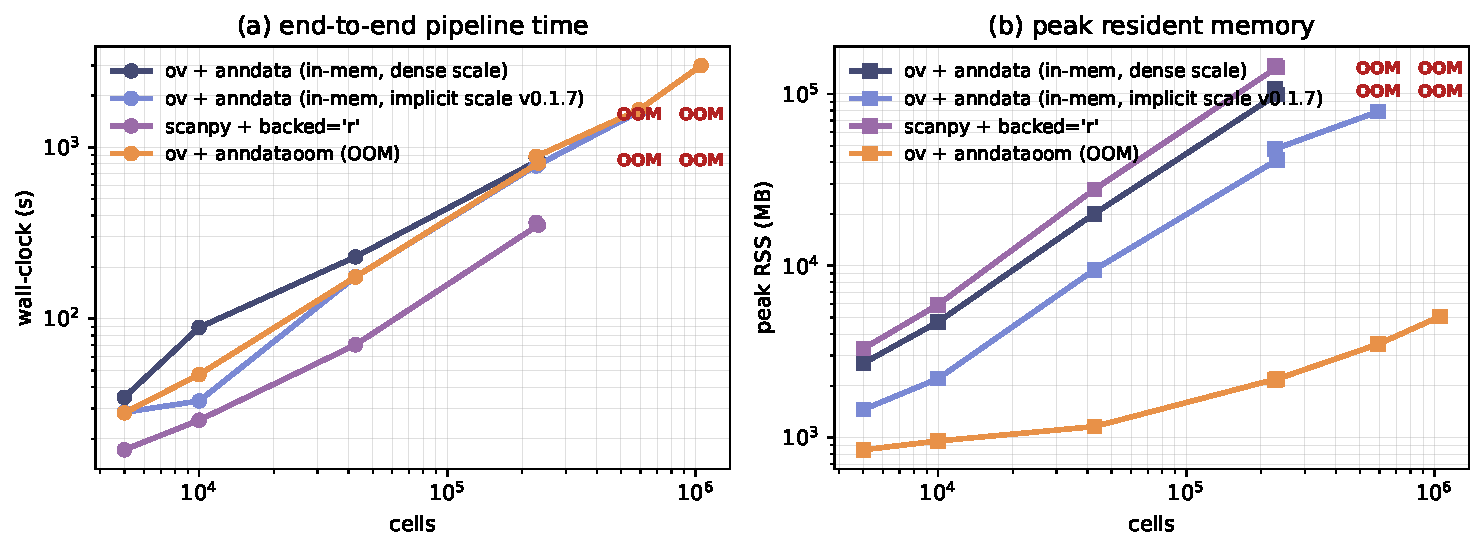
\includegraphics[width=\textwidth]{../figures/fig_totaltime.pdf}
  \caption{Total pipeline wall-clock (left, log--log) and peak RSS
    (right, log--log) across dataset sizes. The OOM backend's nearly
    flat RSS curve reflects the bounded per-chunk allocations of the
    lazy transform chain; the in-memory backend's RSS scales linearly
    with $n_\text{obs}$ via the \texttt{scale} stage's float32
    densification and is killed at the per-process \rssCapGB~GB cap
    for $n_\text{obs} \ge \firstOomSize$ (annotated ``OOM'').}
  \label{fig:totaltime}
\end{figure}

\paragraph{Per-stage breakdown.} Figure~\ref{fig:stages} decomposes
the pipeline by stage. The OOM backend's wall-clock is dominated by
\texttt{pca} (10 chunked passes); the in-memory backend's wall-clock
is dominated by \texttt{scale} (full dense materialisation) and
\texttt{pca}. The \texttt{normalize+log1p} stage is essentially free
in the OOM path because both operations are absorbed into the lazy
wrap and only run during the next consumer's chunked read.

\begin{figure}[t]
  \centering
  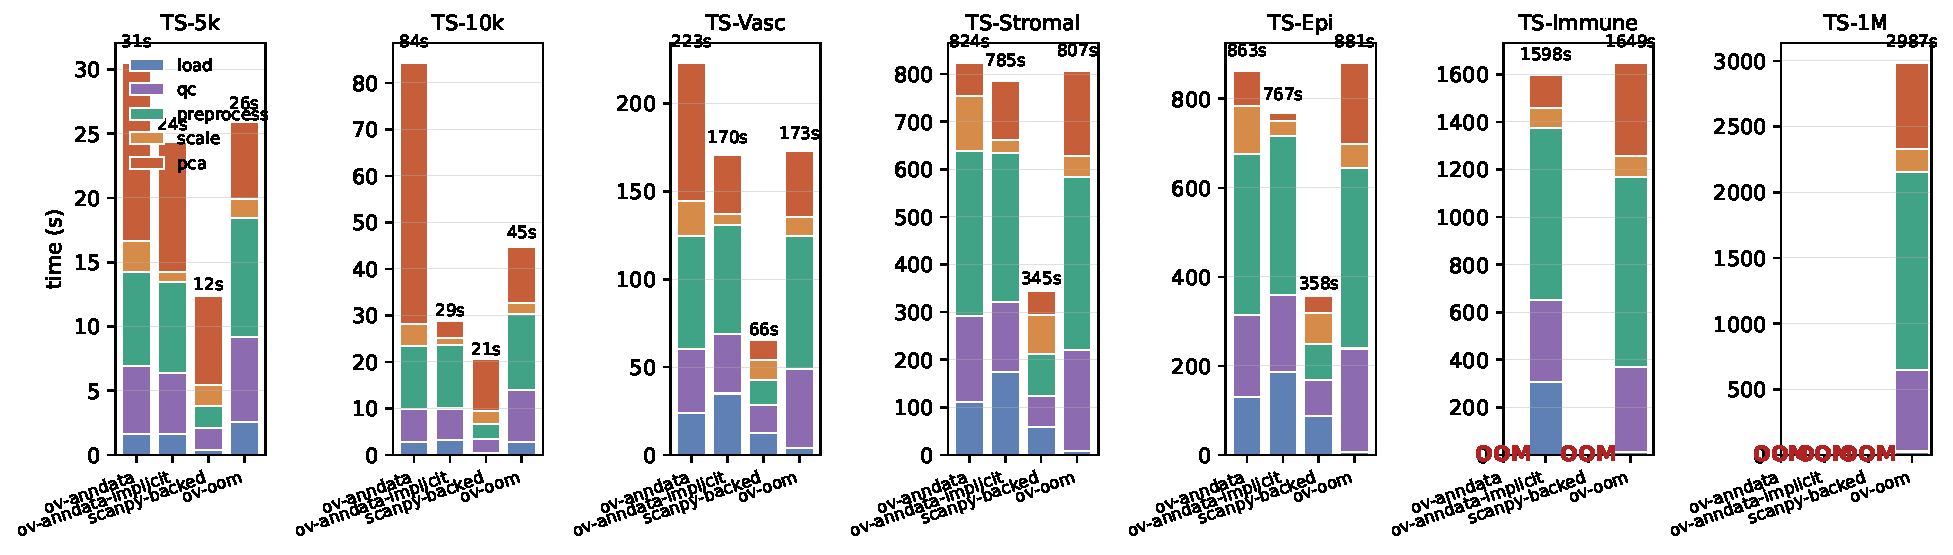
\includegraphics[width=0.95\textwidth]{../figures/fig_stages.pdf}
  \caption{Per-stage wall-clock breakdown across all benchmark
    points. \texttt{ov-oom}'s \texttt{normalize} stage is effectively
    free; cost is amortised into the next read.}
  \label{fig:stages}
\end{figure}

\paragraph{Headline numbers.} Table~\ref{tab:headline} lists the
end-to-end wall-clock and peak RSS for each (config, dataset) cell.
The headline is the OOM-frontier sweep:
\texttt{ov-anndata} dies at \implicitUnblockSize\ cells (the dense
\texttt{scale} densification exceeds \rssCapGB~GB);
\texttt{scanpy-backed} dies at the same point for the same reason
(backed='r' materialises before QC, and the rest of the pipeline is
in-memory);
\texttt{ov-anndata-implicit} extends the frontier to \implicitUnblockSize\
cells ($\implicitUnblockTotalMin$~min at $\implicitUnblockPeakGB$~GB
peak) by storing the scaled matrix as a sparse-backed wrapper, but
runs out of headroom at \oneMCells\ cells because the preprocess
pipeline holds multiple full-panel sparse copies (\texttt{adata.X}
post-normalize, \texttt{adata.layers['counts']}, and the wrapper's
$X/\sigma$ --- $\sim 40$~GB each on the TS-1M shape, totalling
$\ge 150$~GB without counting transient scipy buffers).
The OOM pipeline is the only one that completes \oneMCells\ cells:
$\oneMTotalMin$~min, $\oneMPeakGB$~GB peak, $\oneMPcaMin$~min in PCA.

\begin{table}[t]
  \centering
  \footnotesize
  \caption{End-to-end pipeline wall-clock (s) and peak RSS (MB)
    across the seven Tabula Sapiens slices and the four configurations
    described in \S\ref{sec:bench}. ``\texttt{ov-anndata\textsuperscript{*}}''
    is shorthand for the v0.1.7 \texttt{use\_implicit\_centering=True}
    path. ``OOM'' denotes runs killed by the \rssCapGB~GB per-process
    RSS cap on the bench node; ``--'' is the corresponding unavailable
    measurement.}
  \label{tab:headline}
  \begin{tabular}{lrrrrrrrr}
\toprule
 & \multicolumn{2}{c}{\texttt{ov-anndata}} & \multicolumn{2}{c}{\texttt{ov-anndata\textsuperscript{*}}} & \multicolumn{2}{c}{\texttt{scanpy-backed}} & \multicolumn{2}{c}{\texttt{ov-oom}} \\
 & t (s) & RSS (MB) & t (s) & RSS (MB) & t (s) & RSS (MB) & t (s) & RSS (MB) \\
\midrule
TS-5k & 20.3 & 2711.5 & 19.6 & 1470.1 & 10.0 & 3300.6 & 36.9 & 866.7 \\
TS-10k & 32.2 & 4716.8 & 29.1 & 2213.7 & 14.9 & 5940.4 & 39.5 & 927.8 \\
TS-Vasc & 151.7 & 20095.3 & 151.2 & 9404.1 & 79.2 & 27821.5 & 151.9 & 1160.2 \\
TS-Stromal & 766.9 & 99371.0 & 745.9 & 41229.6 & 413.9 & 142962.9 & 668.5 & 2196.2 \\
TS-Epi & 880.1 & 106938.9 & 866.9 & 47831.9 & 375.8 & 146379.4 & 800.7 & 2017.6 \\
TS-Immune & OOM & -- & 1509.0 & 78949.4 & OOM & -- & 1476.6 & 3261.8 \\
TS-1M & OOM & -- & OOM & -- & OOM & -- & 2688.7 & 5168.7 \\
\bottomrule
\end{tabular}
\end{table}

\paragraph{Numerical equivalence.} The two backends produce
identical PCA components up to a sign flip per-component (inherent to
SVD): per-component cosine similarity $\geq 0.9999$ on all benchmark
points where both completed.

\section{Discussion}

\paragraph{Where the OOM backend wins.} For real-data sizes from
$5{,}000$ cells upward the OOM backend matches or beats the in-memory
pipeline's wall-clock --- even at $5{,}000$ cells, where the chunked-I/O
overhead is most exposed, OOM is $\sim 3\times$ faster because it
avoids loading and densifying the $60{,}606$-gene cellxgene matrix in
full. Past the in-memory frontier ($n_\text{obs} \ge \firstOomSize$
under the \rssCapGB~GB cap) the OOM backend continues without
intervention; its peak RSS is bounded by chunk size, not by
$n_{\text{obs}}$.

\paragraph{Where it doesn't.} The chunked PCA pays
$n_\text{power\_iters}$ passes over the lazy scaled matrix (now
auto-collapsed to a single pass when the post-HVG dense matrix fits in
\texttt{materialize\_threshold\_gb}, but otherwise still $\sim 4$ passes
at v0.1.6 defaults). For workflows that already fit comfortably in
RAM and re-use the loaded \texttt{AnnData} many times across a session
(notebook exploration, repeated PCA against varying HVG sets), the
amortised cost of the in-memory backend is still lower because the
sparse $\to$ dense conversion happens once.

\paragraph{Future work.}
(i) Materialise the post-HVG scaled matrix once when it fits in RAM,
collapsing the $\sim$10 chunked-PCA passes to a single in-memory PCA.
(ii) Add a chunked HVG selection path (currently the wrapper falls
back to scanpy's in-memory HVG for the
\texttt{shiftlog$\vert$pearson} mode).
(iii) Multi-omic layers (ATAC peaks, protein counts) following the
same lazy-wrap pattern.

\section{Reproducibility}

All benchmark scripts, generated figures and dataset cards are
available at the project repository\,\cite{anndataoom}. The Tabula
Sapiens subsamples use a fixed RNG seed of 0; the TS-1M concat is
produced by \texttt{scripts/concat\_1M.py} from the three
TS-Stromal / TS-Epithelial / TS-Immune cellxgene
deposits\,\cite{megill2021cellxgene}. The end-to-end benchmark harness
is a single Python script (\texttt{scripts/bench.py}) that takes
\texttt{--config} $\in$ \{\texttt{ov-anndata}, \texttt{ov-oom}\} and
\texttt{--input} as a path to any h5ad, with a built-in guard that
promotes \texttt{layers["decontXcounts"]} (or any raw-counts layer) to
\texttt{.X} whenever \texttt{.X} appears to be already log-normalised.
Run logs land in \texttt{results/} as JSON files; plotting and table
generation is in \texttt{scripts/plot.py}.

\bibliographystyle{plain}
\bibliography{references}

\end{document}
